\documentclass[conference]{IEEEtran}
\IEEEoverridecommandlockouts
\usepackage{matlab-prettifier}
\usepackage{cite}
\usepackage{amsmath,amssymb,amsfonts}
\usepackage{algorithmic}
\usepackage{graphicx}
\usepackage{textcomp}
\usepackage{xcolor}
\usepackage{float}
\def\BibTeX{{\rm B\kern-.05em{\sc i\kern-.025em b}\kern-.08em
    T\kern-.1667em\lower.7ex\hbox{E}\kern-.125emX}}

\begin{document}

\title{Project 4 : Order Statistics}

\author{\IEEEauthorblockN{Owen Sowatzke}
\IEEEauthorblockA{\textit{Electrical Engineering Department} \\
\textit{University of Arizona}\\
Tucson, USA \\
osowatzke@arizona.edu}}
\maketitle

\begin{abstract}
Consider the set of N iid random variables $\{X_1,...,X_N\}$. The set of random variables can be sorted in ascending order to form a ordered list of random variables $\{X_{(1)},...,X_{(N)}\}$. The n-th ordered statistic is the random variable $X_{(n)}$. This paper derives the pdf of the first-order statistic $X_{(1)}$ and the pdf of the Nth-order statistic $X_{(N)}$. Then, the results are generalized to form the overall order statistics (the pdf of the nth-order statistic $X_{(n)}$ where $N\in [1, N]$).
\end{abstract}

\begin{IEEEkeywords}
Random Variables, Ordered Statistics, Probability Density Function, Cumulative Distribution Function
\end{IEEEkeywords}

\section{Introduction}
Consider N random variables $\{X_1,...,X_N\}$ that are iid with pdf $f_X(x)$. The set of random variables are sorted in ascending order to produce the ordered set of random variable $\{X_{(1)},...,X_{(N)}\}$. The first order statistic is defined as the following:
\begin{equation}
X_{(1)}\triangleq\text{min}\{X_1,...,X_N\}
\end{equation}
Similarly, the Nth-order statistic is defined as the following:
\begin{equation}
X_{(N)}\triangleq\text{max}\{X_1,...,X_N\}
\end{equation}
In this document, the pdf of the first-order statistic $f_{X_{(1)}}(x)$ and the pdf of the Nth-order statistic $f_{X_{(N)}}(x)$ are derived. Finally, the pdf of the overall order statistics is derived (i.e. $f_{X_{(n)}}(x)$ for any $n\in[1,N]$).
%(the pdf of $X_{(n)} \quad \forall n \in[1, N]$) are derived.
% $\triangleq\text{min}\{X_1,...,X_N\}$


%The goal in this section is to derive pdfs for the minimum $X_{(1)}=\text{min}(X_1,...,X_N)$ (called the first-order statistic), the maximum $X_{(1)}=\text{max}(X_1,...,X_N)$ (called the N-th order statistic), as well as the overall order statistics. 
%Sort these variables in ascending order. If the random variables are sorted in increasing order, the   

%Suppose N random variables are drawn from the distribution of the random variable X {
%
%The order statistics of a random variable are defined as the pdf.
\section{First-Order Statistic}

\label{First-Order Statistic Section}

%% Orignal Code
%The cdf of the first-order statistic is given by
%\begin{equation}
%F_{X_{(1)}}(x) = P(\{X_{(1)} \leq x\})
%\end{equation}
%Note that there are many ways for $X_{(1)}$ to be less than or equal to $x$. To simplify this problem, $F_{X_{(1)}}(x)$ can be expressed in the following form:
%\begin{equation}
%F_{X_{(1)}}(x) = 1 - P(\{X_{(1)} > x\})
%\end{equation}
%For $X_{(1)}$ to be greater than $x$, each $X$ ($X_1,...,X_N$) must be greater than $x$.
%\begin{equation}
%F_{X_{(1)}}(x) = 1 - P(\{X_1 > x \} \cap \cdots \cap \{X_N > x \})
%\end{equation}
%Because $X_1,...,X_N$ are independent with the same distribution, the cdf can be expressed in the following form:
%\begin{equation}
%F_{X_{(1)}}(x) = 1 - [P(\{X > x\})]^N
%\end{equation}
%$P(\{X > x\})$ can be rewritten in terms of $F_X(x)$. This provides the following result:
%\begin{equation}
%\label{1st order cdf}
%F_{X_{(1)}}(x) = 1 - [1 - F_X(x)]^N
%\end{equation}
%The pdf of the first order statistic is the derivative of the cdf given in equation \eqref{1st order cdf}.
%\begin{equation}
%F_{X_{(1)}}(x) = -N[1 - F_X(x)]^{N-1}(-f_X(x))
%\end{equation}
%After simplifying the derivative, the pdf of the first order statistic can be written as follows:
%\begin{equation}
%f_{X_{(1)}}(x) = N[1 - F_X(x)]^{N-1}f_X(x)
%\end{equation}


%% New Code
The cumulative distribution function (cdf) of the first-order statistic can be expressed as follows:
\begin{equation}
F_{X_{(1)}}(x) = P(\{X_{(1)} \leq x\})
\end{equation}
%  is smaller than or equal to $x$,
If $X_{(1)} \leq x$, not much can be said about $X_{(2)},...,X_{(N)}$. These random variables can be larger than or smaller than $x$ and still provide $X_{(1)} \leq x$. However, the cdf of the first-order statistic can be expressed in a more useful form as follows:
\begin{equation}
F_{X_{(1)}}(x) = 1 - P(\{X_{(1)} > x\})
\end{equation}
If $X_{(1)} > x$, $X_{(2)},...,X_{(N)}$ are also greater than $x$. Therefore, if  $X_{(1)} > x$, each of the random variables $X_1,...,X_N$ must be greater than $x$. 
\begin{equation}
F_{X_{(1)}}(x) = 1 - P\left(\bigcap_{i=1}^N\{X_i > x\}\right)
\end{equation}
Because the random variables $X_1,...,X_N$ are independent, the cdf of the first-order statistic can be written as follows:
\begin{equation}
F_{X_{(1)}}(x) = 1 - \prod_{i=1}^N P(\{X_i > x\})
\end{equation}
This equation can be rewritten in terms of the distribution functions $F_{X_1}(x),...,F_{X_N}(x)$ as follows:
\begin{equation}
\begin{gathered}
F_{X_{(1)}}(x) = 1 - \prod_{i=1}^N (1-P(\{X_i \leq x\}))\\
= 1 - \prod_{i=1}^N (1-F_{X_i}(x))
\end{gathered}
\end{equation}
Each of the random variables $X_1,...,X_N$ has the same distribution.
\begin{equation}
F_{X_1}(x)=\cdots=F_{X_N}(x)=F_X(x)
\end{equation}
Therefore, the cdf of the first-order statistic can be expressed as follows: 
\begin{equation}
F_{X_{(1)}}(x) = 1 - [1 - F_X(x)]^N
\end{equation}
The probability density function (pdf) of the first-order statistic is the derivative of the cdf with respect to $x$.
\begin{equation}
f_{X_{(1)}}(x) = \frac{d}{dx}\left\{F_{X_{(1)}}(x)\right\}
\end{equation}
Solving for the derivative, the following equation results:
\begin{equation}
f_{X_{(1)}}(x) = -N[1 - F_X(x)]^{N-1}(-f_X(x))
\end{equation}
Finally, after simplifying, the pdf of the first-order statistic can be expressed as follows:
\begin{equation}
f_{X_{(1)}}(x) = N[1 - F_X(x)]^{N-1}f_X(x)
\end{equation}
\section{Nth-Order Statistic}
\label{Nth-Order Statistic Section}

% Original Code
%The cdf of the Nth-order statistic is given by
%\begin{equation}
%F_{X_{(N)}}(x) = P(\{X_{(N)} \leq x\})
%\end{equation}
%For $X_{(N)}$ to be less than or equal to $x$, each $X$ ($X_1,...,X_N$) must be less than or equal to $x$.
%\begin{equation}
%F_{X_{(N)}}(x) = P(\{X_1 \leq x \} \cap \cdots \cap \{X_N \leq x \})
%\end{equation}
%Because $X_1,...,X_N$ are independent with the same distribution, the cdf can be expressed in the following form:
%\begin{equation}
%F_{X_{(N)}}(x) = [P(\{X \leq x \}]^N
%\end{equation}
%Substituting $F_X(x)$ for $P(\{X \leq x \}$, the cdf is given by the following:
%\begin{equation}
%\label{Nth order cdf}
%F_{X_{(N)}}(x) = [F_X(x)]^N
%\end{equation}
%The pdf of the Nth-order statistic is the derivative of the cdf given in equation \eqref{Nth order cdf}. After taking the derivative, the following result ensues.
%\begin{equation}
%f_{X_{(N)}}(x) = N[F_X(x)]^{N-1}f_X(x)
%\end{equation}

% New Code
The cdf of the Nth-order statistic function can be expressed as follows:
\begin{equation}
F_{X_{(N)}}(x) = P(\{X_{(N)} \leq x\})
\end{equation}
If $X_{(N)} \leq x$, $X_{(1)},...,X_{(N-1)}$ are also less than or equal to $x$. Therefore, if  $X_{(N)} \leq x$, each of the random variables $X_1,...,X_N$ must be less than or equal to $x$.
\begin{equation}
F_{X_{(N)}}(x) = P\left(\bigcap_{i=1}^N\{X_i \leq x\}\right)
\end{equation}
Because the random variables $X_1,...,X_N$ are independent, the cdf of the Nth-order statistic can be written as follows:
\begin{equation}
F_{X_{(N)}}(x) = \prod_{i=1}^N P(\{X_i \leq x\})
\end{equation}
This equation can be rewritten in terms of the distribution functions $F_{X_1}(x),...,F_{X_N}(x)$ as follows:
\begin{equation}
F_{X_{(N)}}(x) = \prod_{i=1}^N F_{X_i}(x)
\end{equation}
Because each of the random variables has the same distribution function, the cdf of Nth-order statistic function, can be expressed as follows:
\begin{equation}
F_{X_{(N)}}(x) = [F_X(x)]^N
\end{equation}
The pdf of the Nth-order statistic can be found by differentiating the cdf with respect to x. Solving for the derivative, the following equation results:
\begin{equation}
f_{X_{(N)}}(x) = N[F_X(x)]^{N-1}f_X(x)
\end{equation}
\section{Overall order Statistics}
The results from Section \ref{First-Order Statistic Section} and \ref{Nth-Order Statistic Section} can be generalized, to provide the pdf for nth-order statistic where $n\in[1,N]$. The pdf of the nth-order statistic function can be derived using the cdf of the nth-order statistic function. The cdf is given by the following equation:
\begin{equation}
F_{X_{(n)}}(x) = P(\{X_{(n)} \leq x\})
\end{equation}
Define the events $A_1$ and $A_2$ as follows:
\begin{equation}
A_1 = \{X \leq x\}
\end{equation}
\begin{equation}
A_2 = \{X > x\}
\end{equation}
The probability that there are exactly $k$ occurrences of $A_1$ and $N-k$ occurrences of $A_2$ is given by
\begin{equation}
P_n(k) = \binom{N}{k}[P(A_1)]^k[P(A_2)]^{N-k}
\end{equation}
For $X_{(n)} \leq x$, there must be at least n occurrences of event $A_1$. The number of occurrences of event $A_2$ can range from $N-n$ downto $0$. Since these events are disjoint, they can be expressed as a sum of probabilities.
\begin{equation}
\label{prob sum}
F_{X_{(n)}}(x) = \sum_{k=n}^{N}\binom{N}{k}[P(A_1)]^k[P(A_2)]^{N-k}
\end{equation}
The probability of events $A_1$ and $A_2$ are given by the following equations:
\begin{equation}
P(A_1) = P(\{X \leq x\}) = F_X(x)
\end{equation}
\begin{equation}
P(A_2) = P(\{X > x\}) = 1 - F_X(x)
\end{equation}
Substituting these probabilities into equation \eqref{prob sum}, the cdf of the nth-order statistic can be written as follows:
\begin{equation}
F_{X_{(n)}}(x) = \sum_{k=n}^{N}\binom{N}{k}[F_X(x)]^k[1-F_X(x)]^{N-k}
\end{equation}
The pdf of the nth-order statistic can be found by differentiating the cdf with respect to $x$. The resulting pdf is given by the following equation:
\begin{equation}
\begin{gathered}
f_{X_{(n)}}(x) = \sum_{k=n}^{N}\binom{N}{k}k[F_X(x)]^{k-1}f_X(x)[1-F_X(x)]^{N-k}\\
 + \sum_{k=n}^{N}\binom{N}{k}[F_X(x)]^{k}(N-k)[1-F_X(x)]^{N-k-1}(-f_X(x))
\end{gathered}
\end{equation}
The second summation is 0 when $k=N$. After removing this final term and simplifying the equation, the pdf of the nth-order statistic can written as follows:
\begin{equation}
\begin{gathered}
f_{X_{(n)}}(x) = f_X(x)\sum_{k=n}^{N}\binom{N}{k}k[F_X(x)]^{k-1}[1-F_X(x)]^{N-k}\\
- f_X(x)\sum_{k=n}^{N-1}\binom{N}{k}(N-k)[F_X(x)]^{k}[1-F_X(x)]^{N-k-1}
\end{gathered}
\end{equation}
If the binomial coefficients are expanded, the resulting pdf can be further reduced:
\begin{equation}
\begin{gathered}
f_{X_{(n)}}(x) = f_X(x)\sum_{k=n}^{N}\frac{N!}{k!(N-k)!}k[F_X(x)]^{k-1}\\
\cdot[1-F_X(x)]^{N-k} - f_X(x)\sum_{k=n}^{N-1}\frac{N!}{k!(N-k)!}\\
\cdot(N-k)[F_X(x)]^{k}[1-F_X(x)]^{N-k-1}
\end{gathered}
\end{equation}
After canceling terms in the numerator of the expanded binomial coefficients, the following equation results:
\begin{equation}
\begin{gathered}
f_{X_{(n)}}(x) = f_X(x)\sum_{k=n}^{N}\frac{N!}{(k-1)!(N-k)!}[F_X(x)]^{k-1}\\
\cdot[1-F_X(x)]^{N-k} - f_X(x)\sum_{k=n}^{N-1}\frac{N!}{k!(N-k-1)!}\\
\cdot[F_X(x)]^{k}[1-F_X(x)]^{N-k-1}
\end{gathered}
\end{equation}
After rearranging terms, the equation can be reexpressed as follows:
\begin{equation}
\begin{gathered}
f_{X_{(n)}}(x) = f_X(x)\sum_{k=n}^{N}\frac{N(N-1)!}{(k-1)!(N-k)!}[F_X(x)]^{k-1}\\
\cdot[1-F_X(x)]^{N-k} - f_X(x)\sum_{k=n}^{N-1}\frac{N(N-1)!}{k!(N-k-1)!}\\
\cdot[F_X(x)]^{k}[1-F_X(x)]^{N-k-1}
\end{gathered}
\end{equation}
This equation can be rewritten in terms of binomial coefficients.
\begin{equation}
\begin{gathered}
f_{X_{(n)}}(x) = Nf_X(x)\sum_{k=n}^{N}\binom{N-1}{k-1}[F_X(x)]^{k-1}\\
\cdot[1-F_X(x)]^{N-k} - Nf_X(x)\sum_{k=n}^{N-1}\binom{N-1}{k}\\
\cdot[F_X(x)]^{k}[1-F_X(x)]^{N-k-1}
\end{gathered}
\end{equation}
If $m$ is define as $k-1$, the first summation can be rewritten as:
\begin{equation}
\begin{gathered}
f_{X_{(n)}}(x) = Nf_X(x)\sum_{m=n-1}^{N-1}\binom{N-1}{m}[F_X(x)]^{m}\\
\cdot[1-F_X(x)]^{N-m-1} - Nf_X(x)\sum_{k=n}^{N-1}\binom{N-1}{k}\\
\cdot[F_X(x)]^{k}[1-F_X(x)]^{N-k-1}
\end{gathered}
\end{equation}
After the second sum is subtracted from the first, all that remains is the first term of the first summation.
\begin{equation}
f_{X_{(n)}}(x) = Nf_X(x)\binom{N-1}{n-1}[F_X(x)]^{n-1}[1-F_X(x)]^{N-n}
\end{equation}
Finally, the pdf of the nth-order statistic can be expressed using the following equation:
\begin{equation}
\begin{gathered}
f_{X_{(n)}}(x) = \frac{N!}{(n-1)!(N-n)!}\\
\cdot[F_X(x)]^{n-1}[1-F_X(x)]^{N-n}f_X(x)
\end{gathered}
\end{equation}
Substituting $n=1$ and $n=N$, the pdf of the first-order and Nth-order statistic can be confirmed. 
%% Old Material
%The results from Section \ref{First-Order Statistic Section} and \ref{Nth-Order Statistic Section} can be generalized, to provide the pdf for nth-order statistic where $n\in[1,N]$. 
%\begin{figure}[H]
%\centerline{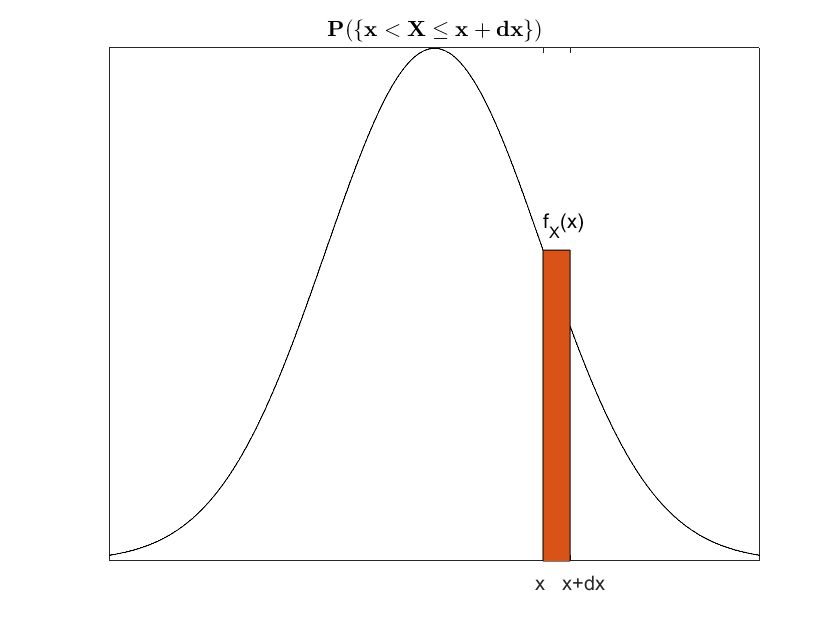
\includegraphics[width=0.5\textwidth]{prob_pdf.png}}
%\caption{Probability that x lies in interval $(x, x+dx]$.}
%\label{Probability of Interval}
%\end{figure}
%\noindent
%Referring to Fig. \ref{Probability of Interval}, the pdf of the n-th order statistic can be expressed in terms of a probability as follows: 
%\begin{equation}
%f_{X_{(n)}}(x)dx = P(\{x < X_{(n)} \leq x+dx\})
%\end{equation}
%For $X_{(n)}$ to lie in interval $(x,x+dx]$, n-1 $X$'s must lie in the interval $(-\infty,x]$, 1 $X$ must lie in the interval $(x,x+dx]$, and N-n $X$'s must lie in the interval $(x+dx,\infty)$. 
%\par
%Let $A_1,A_2,\text{ and }A_3$ be the events that $X$ lies in the intervals $(-\infty,x],(x,x+dx],\text{ and }(x+dx,\infty)$ respectively.
%\begin{equation}
%A_1 = \{X \leq x\}
%\end{equation}
%\begin{equation}
%A_2 = \{x < X \leq x + dx\}
%\end{equation}
%\begin{equation}
%A_3 = \{X > x + dx\}
%\end{equation}
%The probability that $X_{(n)}$ lies in the interval $(x,x+dx]$, can be viewed as taking N samples from the distribution $F_X(x)$. The probability of interest is then the probability of n-1 occurences of $A_1$, 1 occurence of $A_2$, and N-n occurences of $A_3$.
%\begin{equation}
%\begin{gathered}
%P\{x < X_{(n)} \leq x + dx\}=\\
%\frac{N!}{(n-1)!1!(N-n)!}(P(A_1))^{n-1}P(A_2)(P(A_3))^{N-n}
%\end{gathered}
%\end{equation}
%The probabilities of the events $A_1,A_2,\text{ and }A_3$ can be written as follows:
%\begin{equation}
%P(A_1) = P(\{X \leq x\}) = F_X(x)
%\end{equation}
%\begin{equation}
%P(A_2) = P(\{x < X \leq x + dx\}) = f_X(x)dx
%\end{equation}
%\begin{equation}
%P(A_3) = P(\{X > x + dx\}) = 1 - P(\{X \leq x + dx\})
%\end{equation}
%As $dx \rightarrow 0$, $P(\{X \leq x + dx\}) \rightarrow F_X(x)$. Therefore, $P(A_3)$ can be expressed as follows:
%\begin{equation}
%P(A_3) = 1 - F_X(x)
%\end{equation}
%Substituting values for probabilities, the following result can be generated:
%\begin{equation}
%\begin{gathered}
%f_{X_{(n)}}(x)dx=\frac{N!}{(n-1)!1!(N-n)!}\cdot\\
%[F_X(x)]^{n-1}(f_X(x)dx)[1-F_X(x)]^{N-n}
%\end{gathered}
%\end{equation}
%Dividing both sides of the equation by $dx$, the final result can be generated generated:
%\begin{equation}
%\begin{gathered}
%f_{X_{(n)}}(x)=\frac{N!}{(n-1)!(N-n)!}\cdot\\
%[F_X(x)]^{n-1}[1-F_X(x)]^{N-n}f_X(x)
%\end{gathered}
%\end{equation}

%\begin{equation}
%P_n(k_1,...,k_r)=\frac{n!}{k_1! \cdots k_r!}p_1^{k_1} \cdots p_r^{k_r}
%\end{equation}
%%\begin{equation}
%%A_1 = \{X \leq x\}
%%\end{equation}
%%\begin{equation}
%%A_2 = \{x < X \leq x + dx\}
%%\end{equation}
%%\begin{equation}
%%A_3 = \{X > x + dx\}
%%\end{equation}
%\begin{equation}
%P(A_1) = P(\{X \leq x\}) = F_X(x)
%\end{equation}
%\begin{equation}
%P(A_2) = P(\{x < X \leq x + dx\}) = f_X(x)dx
%\end{equation}
%\begin{equation}
%P(A_3) = P(\{X > x + dx\}) = 1 - P(\{X \leq x + dx\})
%\end{equation}
%%The first order statistic is the probability that one of the random variables $X$ falls in the the interval  
%As $dx \rightarrow 0$, $P(\{X \leq x + dx\}) \rightarrow F_X(x)$. Therefore, $P(A_3)$ can be expressed as follows:
%\begin{equation}
%P(A_3) = 1 - F_X(x)
%\end{equation}
%\begin{equation}
%f_{X_{(n)}}(x)dx = P\{x < X_{(n)} \leq x + dx\}
%\end{equation}
%$P\{x < X_{(n)} \leq x + dx\}$ is the probability that 1 $X$ falls in the interval $(x, x+dx]$, $n-1$ $X$'s fall in the interval $(-\infty, x]$, and $N-n$ $X$'s fall in the interval $(x+dx, \infty)$. It can be expressed in the following form:
%\begin{equation}
%\begin{gathered}
%P\{x < X_{(n)} \leq x + dx\}=\\
%\frac{N!}{(n-1)!1!(N-n)!}(P(A_1))^{n-1}P(A_2)(P(A_3))^{N-n}
%\end{gathered}
%\end{equation}
%Substituting values for probabilities, the following result can be generated:
%\begin{equation}
%\begin{gathered}
%f_{X_{(n)}}(x)dx=\frac{N!}{(n-1)!1!(N-n)!}\cdot\\
%[F_X(x)]^{n-1}(f_X(x)dx)[1-F_X(x)]^{N-n}
%\end{gathered}
%\end{equation}
%Dividing both sides of the equation by $dx$, the final result can be generated generated:
%\begin{equation}
%\begin{gathered}
%f_{X_{(n)}}(x)=\frac{N!}{(n-1)!(N-n)!}\cdot\\
%[F_X(x)]^{n-1}[1-F_X(x)]^{N-n}f_X(x)
%\end{gathered}
%\end{equation}
%
%
%The pdf of the first order statistic $X_{(1)}$ can be defined as follows:
%\begin{equation}
%f_{X_{(1)}}(x)=\frac{P(\{x < X_{(1)} \leq x+dx\})}{dx}
%\end{equation}
%After rearranging terms, the equation can be expressed as follows:
%\begin{equation}
%f_{X_{(1)}}(x)dx=P(\{x < X_{(1)} \leq x+dx\})
%\end{equation}
%If $X_k$ is the smallest random variable 
%\begin{equation}
%P(\{x < X_k \leq x+dx\} \cap \{X_i > x+dx\}) \quad \forall i \neq k 
%\end{equation}
%%\section{N-th order Statistic}
\section{Conclusion}
%Both Monte Carlo (MC) Simulations and Importance Sampling (IS) are techniques for estimating probabilities. In this document, both techniques will be used to estimate the probability that a random variable $X$ with distribution $X\sim N(1,1)$ exceeds 3.957 (i.e. $P\{X > 3.957\}$).
%\section{Monte Carlo Simulation}
%The probability of interest can be written as follows:
%\begin{equation}
%P\{X > 3.957\} = \int_{-\infty}^{\infty}I(x)f_X(x)dx
%\label{Pint}
%\end{equation}
%where
%\begin{equation}
%I(x) = \begin{cases}
%1 & x > 3.957 \\
%0 & x \leq 3.957
%\end{cases}
%\label{Ix_def}
%\end{equation}
%Note that this probability can also be written as an expected value:
%\begin{equation}
%P\{X > 3.957\} = E[I(X)]
%\end{equation}
%Monte Carlo Simulation attempts to estimate this probability using a sample mean
%\begin{equation}
%P\{X > 3.957\} \approx \frac{1}{N}\sum_{i=1}^{N}I(x_i)
%\end{equation}
%where
%\begin{equation}
%x_1, x_2, ..., x_N \sim f_X(x)
%\end{equation}
%\par
%Given different values of $N \in [1, 10^5]$, Monte Carlo Simulations can be used to estimate $P\{X > 3.957\}$. This estimate can than be compared to the true probability.
%\begin{equation}
%P\{X > 3.957\} = 0.001553
%\end{equation}
%The Monte Carlo probability estimate was generated for values $N$ from $100$ to $10^5$ in increments of $100$. The MATLAB code to generate this estimate is included in Appendix \ref{matlab_code}. The Monte Carlo probability estimate is plotted vs $N$ in Fig. \ref{Monte Carlo Estimate}
%\begin{figure}[H]
%\centerline{\includegraphics[width=0.5\textwidth]{Monte_Carlo_Estimate.png}}
%\caption{Monte Carlo Probability Estimate}
%\label{Monte Carlo Estimate}
%\end{figure}
%\noindent
%The absolute value of the error between the Monte Carlo estimate and the true probability ($|P_{est}\{X > 3.957\} - P_{truth}\{X > 3.957\}|$) is also plotted vs $N$.
%\begin{figure}[H]
%\centerline{\includegraphics[width=0.5\textwidth]{Monte_Carlo_Error.png}}
%\caption{Monte Carlo Probability Error}
%\label{Monte Carlo Perr}
%\end{figure}
%As $N\rightarrow\infty$, the Monte Carlo Estimate should approach the true probability. This is confirmed by examining the results shown in Fig. \ref{Monte Carlo Perr}.
%\section{Importance Sampling}
%Examining the shaded area shown in Fig. 
%\ref{Monte Carlo Limits}, very few of the samples from $f_X(x)$ contribute to the Monte Carlo probability estimate. This leads to large variances in the estimated probability.
%\begin{figure}[H]
%\centerline{\includegraphics[width=0.5\textwidth]{MC_Indicator.png}}
%\caption{Important Samples from $f_X(x)$}
%\label{Monte Carlo Limits}
%\end{figure}
%Importance Sampling attempts to overcome these limitations. It re-expresses equation \eqref{Pint} in the following form:
%\begin{equation}
%P\{X > 3.957\} = \int_{-\infty}^{\infty}I(x)f_X(x)\frac{g_X(x)}{g_X(x)}dx
%\label{is_int}
%\end{equation}
%where $I(x)$ is given by equation \eqref{Ix_def}.
%Equation \eqref{is_int} can be also be written as follows:
%\begin{equation}
%P\{X > 3.957\} = \int_{-\infty}^{\infty}\left[I(x)\frac{f_X(x)}{g_X(x)}\right]g_X(x)dx
%\end{equation}
%This equation also represents an expected value.
%\begin{equation}
%P\{X > 3.957\} = E\left[I(x)\frac{f_X(x)}{g_X(x)}\right]
%\end{equation}
%Once again, the expected value can be estimated using a sample mean.
%\begin{equation}
%P\{X > 3.957\} \approx \frac{1}{N}\sum_{i=1}^{N}I(x_i)\frac{f_X(x_i)}{g_X(x_i)}
%\label{is_prob_est}
%\end{equation}
%Note the samples $x_1,x_2,...,x_N$ are now sampled from $g_X(x)$ instead of $f_X(x)$. As such, the density function $g_X(x)$ can be selected to provide more "important" samples. 
%\par
%Consider a density $g_X(x)$ that is a shifted version of $f_X(x)$. Specifically, consider the following density function
%\begin{equation}
%g_X(x) = \frac{1}{\sqrt{2\pi}}e^{-(x-3.957)^2/2}
%\end{equation}
%The "important" samples of the new density function $g_X(x)$ are highlighted in Fig. \ref{Important Samples}. 
%\begin{figure}[H]
%\centerline{\includegraphics[width=0.5\textwidth]{IS_Indicator.png}}
%\caption{Important Samples from $g_X(x)$}
%\label{Important Samples}
%\end{figure}
%\noindent
%Note that the number of important samples is significantly larger than that of Fig. \ref{Monte Carlo Limits}. This should reduce the variance of the probability estimate. 
%\par
%To confirm this result, an Importance Sampling probability estimate was generated for different values of $N$ using equation \eqref{is_prob_est}. The MATLAB code to generate this estimate is included in Appendix \ref{matlab_code}. The Important Sampling probability estimate is plotted vs $N$ in Fig. \ref{Importance Sampling Estimate}.
%\begin{figure}[H]
%\centerline{\includegraphics[width=0.5\textwidth]{Importance_Sampling_Estimate.png}}
%\caption{Importance Sampling Probability Estimate}
%\label{Importance Sampling Estimate}
%\end{figure}
%\noindent
%The absolute value of the error between the Importance Sampling probability estimate and the true probability ($|P_{est}\{X > 3.957\} - P_{truth}\{X > 3.957\}|$) is also plotted vs $N$.
%\begin{figure}[H]
%\centerline{\includegraphics[width=0.5\textwidth]{Importance_Sampling_Error.png}}
%\caption{Importance Sampling Probability Error}
%\label{Importance Sampling Perr}
%\end{figure}
%The variance of the Monte Carlo and Importance Sampling probability estimates can be compared by overlaying the probability error plots. This plot is shown in Fig. \ref{Error Overlay}
%\begin{figure}[H]
%\centerline{\includegraphics[width=0.5\textwidth]{Error_Overlay.png}}
%\caption{Probability of Error Comparison}
%\label{Error Overlay}
%\end{figure}
%\noindent
%Note that the Importance Sampling probability estimate is much closer to the expected probability than the Monte Carlo Estimate. As such, the Importance Sampling estimate has a lower variance than the Monte Carlo Estimate for the same values of $N$.
%\section{Conclusion}
%Monte Carlo Simulation and Importance Sampling are ways to estimate probabilities. Both of these approaches were used to estimate $P\{X > 3.957\}$ for $X \sim N(1,1)$. As demonstrated, importance sampling produced a probability estimate with a smaller variance than that of Monte Carlo simulation. This result can be applied to other probabilities estimates as well. If a distribution is hard to sample, importance sampling can be used to reduce the number of samples required to produce an estimate. This can make a significant difference, especially when it is computationally intensive to determine the indicator function $I(x)$.
%\onecolumn
%\pagebreak
%\appendices
%\section{MATLAB Source Code}
%\label{matlab_code}
%\lstset{style=Matlab-editor}
%\lstinputlisting{Project3_Sowatzke.m}
%\raggedbottom
\end{document}
